Three of the lensing pipelines (I3, DE, KM) that are included in the
cluster STEP results, also competed in the GREAT10 challenge.
The comparison between the GREAT10 and CSTEP results is shown in 
Figure %\ref{fig:gt10}. The results are roughly consistent between
the two challenges for I3 and KM showing that both pipelines are 
robust, and demonstrate similar levels of shape measurement bias
for a wide variety of sources and PSF types. Both I3 and KM are 
among the best performing lensing pipelines for both CSTEP and
GREAT10. 

\begin{figure}
 \centering  % this centres figure in column
  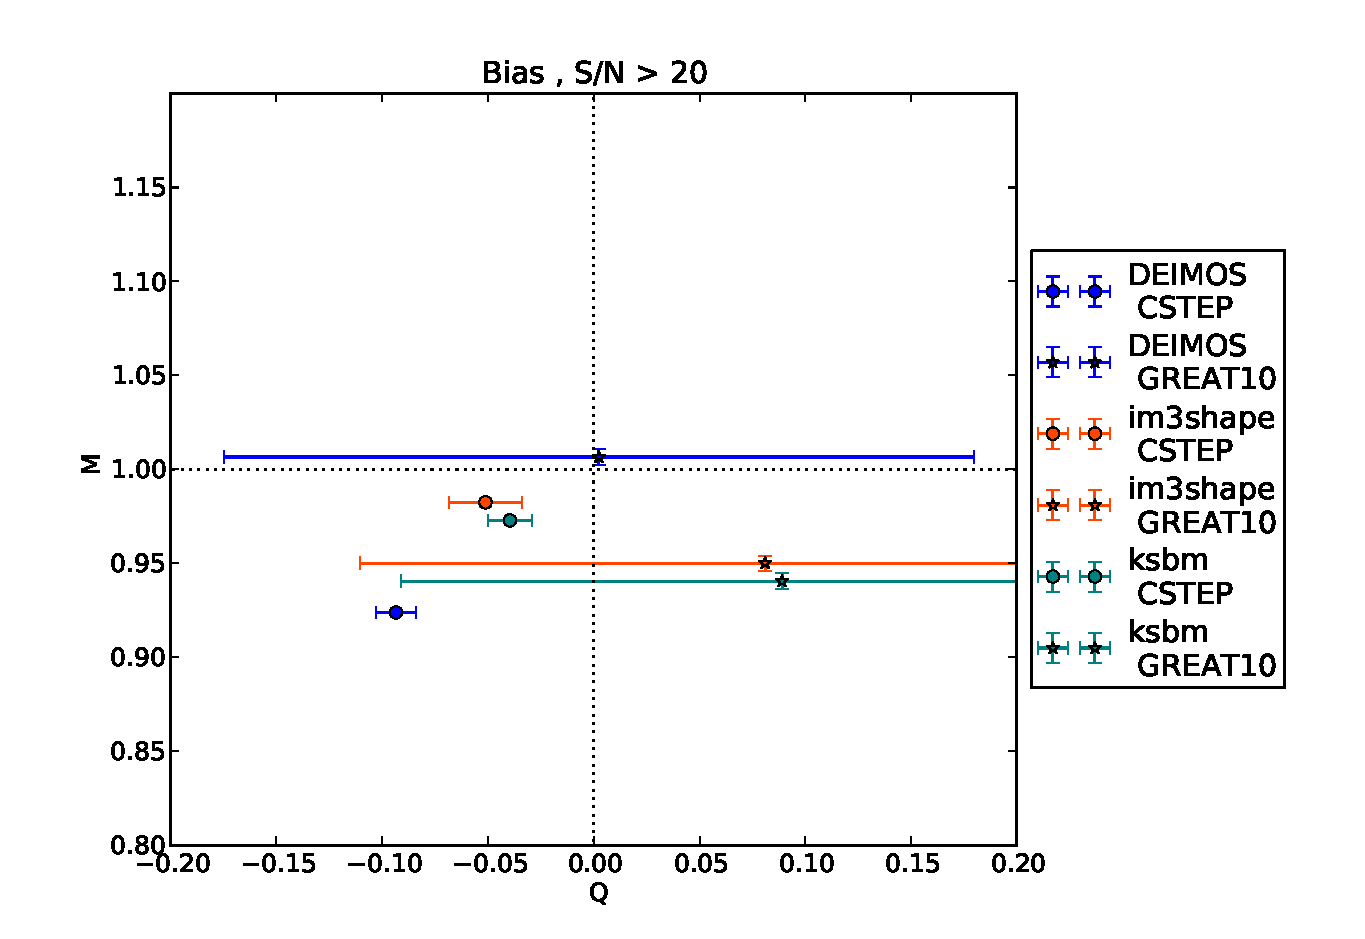
\includegraphics[width=0.45\textwidth]{fig/QMC_gt10.pdf} 
  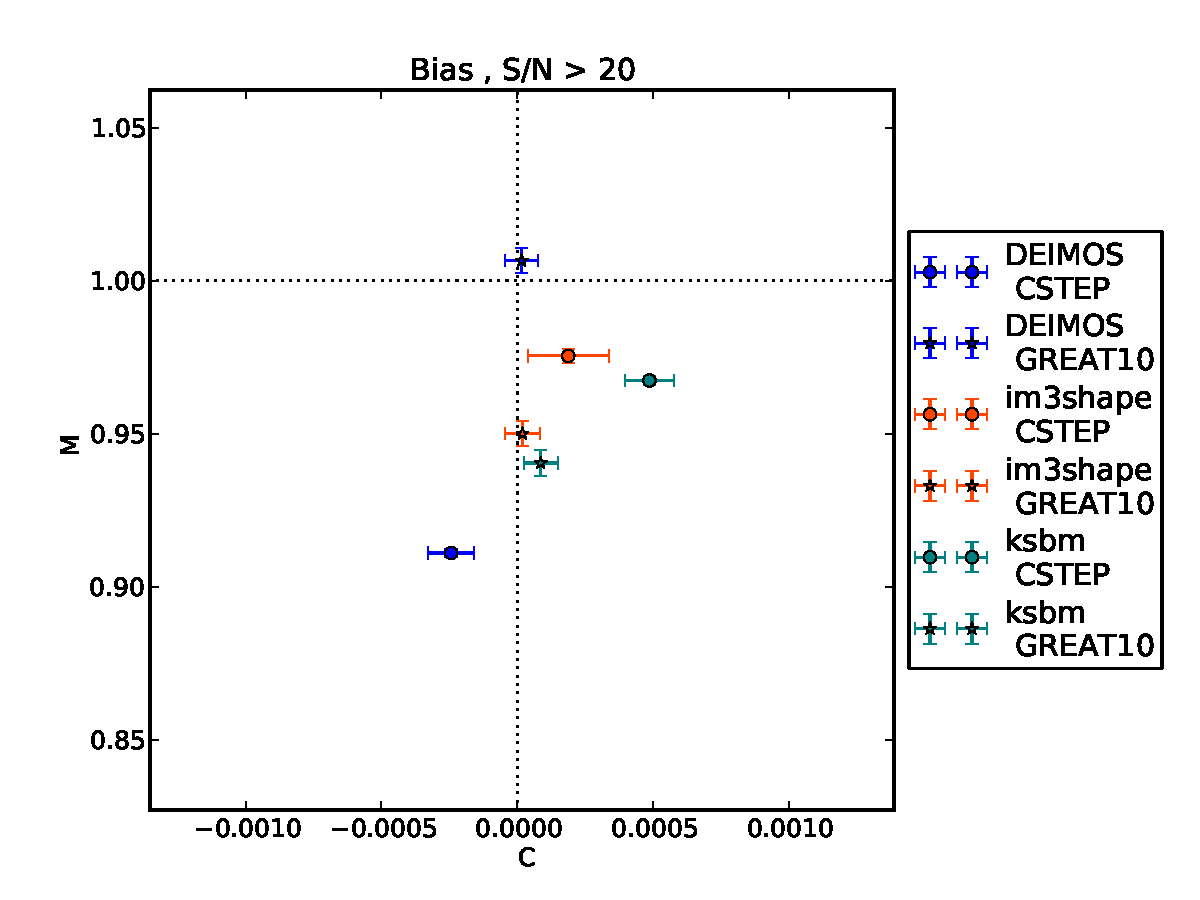
\includegraphics[width=0.45\textwidth]{fig/MC_gt10.pdf} 
  \caption{This figure shows the average shape measurement bias
as measured on all images for galaxy objects SNR $>$ 20 on
CSTEP data and the shape measurement bias as measured by the
same lensing pipelines on the GREAT10 data \citep{GREAT10}. The
top panel shows the shape measurement bias Q,M as measured using 
a Q,M,C fit. The bottom panel shows the shape measurement bias 
M,C as measured using a M,C fit.}
\label{fig:gt10}
\end{figure}

%%%%%%%%%%%%%%%%%%%%%%%%%%%%%%%%%%%%%%%%%%%%%%%%
\begin{table*}
        \centering
        \begin{tabular}{|c|c|c|c|c|c|c|c|}  
          \hline
          Pipeline & Qsel  & Msel  & Csel  & Q  & M  & C  \\
          \hline
          DE & -0.088 $\pm$ 0.017 & 0.928 $\pm$ 0.002 & -0.0014 $\pm$ 0.0002 & -0.094 $\pm$ 0.009 & 0.924 $\pm$ 0.001 & -0.0004 $\pm$ 0.0001 \\
          \hline
          PF & -0.033 $\pm$ 0.040 & 0.988 $\pm$ 0.005 & -0.0004
          $\pm$ 0.0003 & -0.058 $\pm$ 0.038 & 0.963 $\pm$ 0.005 &
          -0.0008 $\pm$ 0.0003 \\
          \hline
          GM & 0.236 $\pm$ 0.032 & 0.944 $\pm$ 0.004 & 0.0006
          $\pm$ 0.0003 & 0.153 $\pm$ 0.034 & 0.991 $\pm$ 0.004 &
          -0.0001 $\pm$ 0.0003  \\
          \hline
          MJ & 0.083 $\pm$ 0.035 & 0.901 $\pm$ 0.004 & 0.0015 $\pm$
          0.0003 & 0.106 $\pm$ 0.043 & 0.867 $\pm$ 0.006 & 0.0016
          $\pm$ 0.0004 & 0.81 \\
          \hline
          PK & -0.029 $\pm$ 0.016 & 0.946 $\pm$ 0.002 & 0.0006 $\pm$
          0.0001 & -0.022 $\pm$ 0.016 & 0.945 $\pm$ 0.002 & 0.0003
          $\pm$ 0.0001 \\
          \hline
          I3 & -0.042 $\pm$ 0.016 & 0.983 $\pm$ 0.002 & 0.0000
          $\pm$ 0.0001 & -0.051 $\pm$ 0.017 & 0.982 $\pm$ 0.002 &
          0.0001 $\pm$ 0.0002 \\
          \hline
          IM & -0.020 $\pm$ 0.058 & 1.275 $\pm$ 0.008 & -0.0066
          $\pm$ 0.0005 & -0.035 $\pm$ 0.066 & 1.098 $\pm$ 0.009 &
          -0.0080 $\pm$ 0.0006 \\
          \hline
          KM & -0.050 $\pm$ 0.010 & 0.981 $\pm$ 0.001 & 0.0007 $\pm$
          0.0001 & -0.040 $\pm$ 0.010 & 0.973 $\pm$ 0.001 & 0.0004
          $\pm$ \\
          \hline
        \end{tabular}
        \caption{ The Q, M, C results for objects SNR $>$ 20. The
          values reported are the reults of a Q,M,C fit after
          correcting for selection effects (Qsel, Msel, Csel) and not
          correcting for selection effects (Q, M, C).}
    \label{table:QMC_sel}
\end{table*}

\begin{table*}
        \centering
        \begin{tabular}{|c|c|c|c|c| }  
          \hline
          Pipeline & Msel  & Csel & M  & C   \\ 
          \hline
          DEIMOS & 0.915 $\pm$ 0.002 & -0.0013 $\pm$ 0.0002 & 0.911
          $\pm$ 0.001 & -0.0002 $\pm$ 0.0001 \\
          \hline
          PFDNT & 0.983 $\pm$ 0.005 & -0.0004 $\pm$ 0.0003 & 0.956
          $\pm$ 0.005 & -0.0007 $\pm$ 0.0003 \\
          \hline
          GaussianMix & 0.976 $\pm$ 0.004 & 0.0003 $\pm$ 0.0003 &
          1.012 $\pm$ 0.004 & -0.0003 $\pm$ 0.0003 \\
          \hline
          MJ & 0.913 $\pm$ 0.004 & 0.0014 $\pm$ 0.0003 & 0.881 $\pm$ 0.006 & 0.0015 $\pm$ 0.0004 \\
          \hline
          PKSB & 0.942 $\pm$ 0.002 & 0.0007 $\pm$ 0.0001 & 0.942 $\pm$
          0.002 & 0.0004 $\pm$ 0.0001 \\
          \hline
          im3shape & 0.977 $\pm$ 0.002 & 0.0001 $\pm$ 0.0001 & 0.975 $\pm$ 0.002 & 0.0002 $\pm$ 0.0002 \\
          \hline
          IMCAT & 1.272 $\pm$ 0.007 & -0.0066 $\pm$ 0.0005  & 1.093 $\pm$ 0.008 & -0.0079 $\pm$ 0.0006 \\
          \hline
          ksbm & 0.975 $\pm$ 0.001 & 0.0008 $\pm$ 0.0001 & 0.967 $\pm$ 0.001 & 0.0005 $\pm$ 0.0001 \\
          \hline
        \end{tabular}
        \caption{ The M, C results for objects SNR $>$ 20. The
          values reported are the reults of a M,C fit after
          correcting for selection effects (Msel, Csel) and not
          correcting for selection effects (M, C).}
    \label{table:MC_sel}
\end{table*}